\section{Kombinatorische Schaltungen}
A combinational circuit outputs, only depend on it's inputs therefore it is memoryless, a sequential circuit output's depend both on it's current and old inputs, it has memory. A combinational circuit has the following properties:
\begin{enumerate}
	\item Every circuit element is combinational.
	\item Every node of the circuit is either designated as an input to the circuit or connects to exactly one output terminal of a circuit element.
	\item The circuit contains no cyclic paths: every path through the circuit visits each circuit node at most once.
\end{enumerate}
	
	\begin{multicols}{2}
	\subsection{Gatter}
		\renewcommand{\arraystretch}{1.5}
		\begin{tabular}{r  || c c c c}
			               &   Logik      &   Algebra                 &   Schaltbild  & Verilog   \\ \hline\hline
		OR		        &   $x \lor y$          &   $x + y$                 
										&   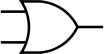
\includegraphics[height = 11pt]{images/gatter/or}    &     \verb+x || y+       \\
		NOR	    &   $\lnot(x \lor y)$    &   $\overline{x + y}$      
										&   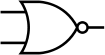
\includegraphics[height = 11pt]{images/gatter/nor}    &                       \\\hline
		AND	         &   $x \land y$        &   $x \cdot y$             
										&   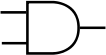
\includegraphics[height = 11pt]{images/gatter/and}    &     \verb+x && y+         \\
		NAND	    &   $\lnot(x \land y)$  &   $\overline{x \cdot y}$  
										&   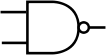
\includegraphics[height = 11pt]{images/gatter/nand}    &                     \\\hline
		NOT	          &   $\lnot x$            &   $\overline{x}$          
										&   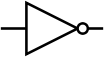
\includegraphics[height = 11pt]{images/gatter/not}    &     \verb+!x+         \\\hline
		XOR	    &   $x \ne y$           &   $x \oplus y$            
										&   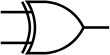
\includegraphics[height = 11pt]{images/gatter/xor}    &     \verb+x ^ y+             \\\hline
		XNOR	        &   $x = y$             &   $\overline{x \oplus y}$ 
										&   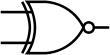
\includegraphics[height = 11pt]{images/gatter/xnor}    &     \verb+x == y+       \\\hline
			       &   $x \to y$           &   $x \le y$        
										&   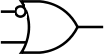
\includegraphics[height = 11pt]{images/gatter/implies}    &   \verb+!x || y+       \\
		\end{tabular}
	
	\subsection{Wahrheitstabellen}
	A literal can have the value of 1, 0, x if it is a illegal value(contention) or z if it's is floating(not yet defined).
		\renewcommand{\arraystretch}{1.2}
		\begin{tabular}{c|c||c|c|c|c|c|c}
			%\hline
			$a$ 	& $b$ & $\lnot a$ 	& $a\land b$& $a\lor b$	& $a\rightarrow b$ 	&$a \leftrightarrow b $& $a \oplus b $\\ \hline \hline
			1 		& 1	& 0			&  1			&  1			& 1						& 1										& 0			  \\ \hline
			1 		& 0	& 0			&  0			&  1			& 0						& 0										& 1			  \\ \hline 
			0 		& 1	& 1			&  0			&  1			& 1						& 0										& 1			  \\ \hline
			0 		& 0	& 1			&  0			&  0			& 1						& 1										& 0			  %\\ \hline
		\end{tabular}
	
	\subsection{Normalformen}
		\begin{itemize}
			\item \textbf{DNF}: Disjunktive Normalform(sum of products)(Formel mit nur $\vee$, $\wedge$ und $\neg$ wo alle mit $\vee$ verbunden sind). In der Wahrheitstabelle können die ``1-Zeilen'' verodert werden. \\ ($0 \to \lnot x, 1 \to x$)
			\begin{itemize}
				\item \textbf{Literal}: negierte oder unnegierte Variable
				\item \textbf{Produktterm}: Konjunktion von Literalen
				\item \textbf{Minterm}: holds all literals with and's
				\item \textbf{Maxterm}: holds all literals with or's
			\end{itemize}
			\item \textbf{KNF}: Konjunktive Normalform(alle mit $\wedge$ verbunden sind). In der Wahrheitstabelle können die ``0-Zeilen'' verundet werden. \\ ($0 \to x, 1 \to \lnot x$)
		\end{itemize}
		
	
	\subsection{Umformungen}
	\begin{center}
	\begin{tabular}{l@{\;=\;}l@{\quad=\;}l}
		$a \oplus b$ & $( a \land  \lnot b) \lor ( \lnot a \land b)$ & $a \overline{b} + \overline{a}b$ \\
		& $ (a \lor b) \land ( \lnot a \lor \lnot b) $ & $ (a+b)(\overline a + \overline b) $ \\
		& $ (a \lor b) \land \lnot(a \land b) $ & $ (a+b) \overline{(ab)} $ \\
	\end{tabular}\\
	P$\neg A$ + PA = P
	\end{center}
	
	\subsection{Bubble pushing}
	You can use bubble pushing to make a figure more readable. To do this push the bubbles from the output to the input.
	The rules of bubble pushing are:
	\begin{enumerate}
		\item Pushing bubbles backward (from the output) or forward (from the inputs) changes the body of the gate from AND to OR or vice versa
		\item Pushing a bubble from the output back to the inputs puts bubbles on all gate inputs.
		\item Pushing bubbles on all gate inputs forward toward the output puts a bubble on the output
	\end{enumerate}
	
	\subsection{Frequenzberechnung(sequential circuits)}
		\begin{align*}
			\text{Zykluszeit:} \quad & t_z \geq t_s+t_p+t_l + t_{skew} \\
			\text{propagation delay:} \quad & t_p \leq t_z - (t_l + t_s + t_{skew}) \\
			\text{propagation delay:} \quad & t_l \geq t_{hold} + t_{skew} - t{ccq}\\
			\text{Max. Frequenz:} \quad & f_{max} = \frac{1}{t_z} = \frac{1}{t_s+t_p+t_l} \\
			t_s: \quad & \text{Setupzeit} \\
			t_p: \quad & \text{Propagierungsdelay der Flipflops} \\
			t_l: \quad & \text{Längster Pfad} \\
			t_{skew}: \quad & \text{Difference between times clock takes to reach registers}\\
			t_{ccq}: \quad & \text{Time in the flip-flop}\\
		\end{align*}
		The propagation delay is the sum of the times threw each logic unit in the longest path.\\
		The contamination delay is the sum of the times threw each logic unit in the shortest path.\\If we look a the result in between these two delays, the result might change value,
		this is called a glitch. If the contamination delay is too large the clock period can be increased.
		Synchronous sequential circuits have a timing specification including the clock-to-Q propagation and contamination delays, tpcq and tccq, and the setup and hold times, tsetup and thold. For correct operation, their inputs must be stable during an aperture time that starts a setup time before the rising edge of the clock and ends a hold time after the rising edge of the clock. The minimum cycle time, Tc, of the system is equal to the propagation delay, tpd, through the combinational logic plus tpcq   tsetup of the register. For correct operation, the contamination delay through the register and combinational logic must be greater than thold. Despite the common misconception to the contrary, hold time does not affect the cycle time.
	
	\subsection{Rechenregeln}
		\renewcommand{\arraystretch}{1.5}
		\begin{tabular}{l r @{  } l}
		Kommutativität      	&   $x \land y$           	& $\equiv$  $y \land y$	\\
									&$x \lor y$   						& $\equiv$  $y \lor x$   \\\hline
		Assoziativität      	&   $x \land (y \land z)$ 	& $\equiv$  $(x \land y) \land z$	\\ 
									&   $x \lor (y \lor z)$  		& $\equiv$  $(x \lor y) \lor z$\\\hline
		Distributivität	  	&	 $x \land (y \lor z)$		& $\equiv$	 $(x \land y) \lor (x \land z)$\\
									&	 $x \lor (y \land z)$		&$\equiv$	 $(x \lor y) \land (x \lor z)$\\\hline
		De'Morgan           	&   $\lnot(x \land y)$  		& $\equiv$  $\lnot x \lor \lnot y$ \\
									&   $\lnot(x \lor y)$  			& $\equiv$  $\lnot x \land \lnot y$\\\hline
		Idempotenz          	&   $x \land x$    				& $\equiv$  $x$\\
									&   $x \lor x$  					& $\equiv$  $x$\\\hline
		Controlling Value   	&   $x \land 0$    				& $\equiv$  $0$\\
									&   $x \lor 1$  					&$\equiv$   $1$\\\hline
		Neutraler Wert      	&   $x \land 1$    				& $\equiv$  $x$\\
									&   $x \lor 0$  					& $\equiv$  $x$\\ \hline
		Doppelte Negation		&	 $\lnot(\lnot x)$				&$\equiv$	 $x$ 
 		\\\hline
 		Abschwächung   &		$x \land y $		& $\equiv$ $x \quad$ wenn $x \Rightarrow y$ \\
 		 & \multicolumn{2}{c}{$y$ schwächer als $x$} \\ \hline
 		Verstärkung   &		$x \lor y $		& $\equiv$	$x \quad$ wenn $y \Rightarrow x$ \\
 		 & \multicolumn{2}{c}{$y$ stärker als $x$} \\ \hline
 		Konsensus   & \multicolumn{2}{c}{ $ x \cdot y + \overline x \cdot z + y \cdot z \equiv  x \cdot y + \overline x \cdot z $ } \\ \hline
 		Shannon-Expansion   & \multicolumn{2}{c}{ $ e \equiv x \land e[1/x] \lor \lnot x \land e[0/x] $ } \\\\
		\end{tabular}
		
		where $e$ is a function and $e[1/x]$ is the function where you replace x by 1. Shannon's expansion tells us that any function can be written with a multiplexer(because a double multiplexer is written with $\neg$ the selector $\wedge$ the first function $\vee$ the selector $\wedge$).
	
	\subsection{Bindung der Operatoren}
		\[ \text{ stärker }\qquad \lnot \quad \land \quad \lor \quad \rightarrow \quad \oplus \quad \leftrightarrow \qquad \text{ schwächer ($\oplus$=xor) } \]
	
	\end{multicols}
	\section{Sequential circuits}
	The outputs of sequential logic depend on both current and prior input values. Hence, sequential logic has memory. The sequential system remebers it's prior inputs in information which is called the state of the system, which is stored in state variables. We are going to build synchronous sequential circuits consisting of com- binational logic and banks of flip-flops containing the state of the circuit, final state machines.\\
	\subsection{Memory}
	A bistable element is an element that has two phases, and holds one bit of info.
	\paragraph{latches} There are two types of latches, the sr latch which can store the data, but is a bit weird and the d latch which can store data, it also has an input clock, when clock is 1, the latch shows it's new updated value, when clock is 0 the latch shows it's old value.
	\paragraph{flip-flop} a D flip-flop is composed of two back to back D latches. It has an input D and an output Q. The D flip-flop copies D to Q on the rising edge of the clock, and remembers its state at all other times.\\ An enabled flip-flop has another input, EN (enable), when EN is TRUE, the enabled flip-flop behaves like an ordinary D flip-flop. When EN is FALSE, the enabled flip-flop ignores the clock and retains its state.\\A resettable flip-flop adds another input called RESET. When RESET is FALSE, the resettable flip-flop behaves like an ordinary D flip-flop. When RESET is TRUE, the resettable flip-flop ignores D and resets the output to 0. Such flip-flops may be synchronously or asynchronously resettable. Synchronously resettable flip-flops reset themselves only on the rising edge of CLK. Asynchronously resettable flip-flops reset themselves as soon as RESET becomes TRUE, independent of CLK.
	\paragraph{registers}, a registor has n flip-flops that all have the same CLK, so that all the bits are updated at the same time.
	\\Remember that a D latch is level-sensitive, whereas a D flip-flop is edge-triggered. The D latch is transparent when CLK   1, allowing the input D to flow through to the output Q. The D flip-flop copies D to Q on the rising edge of CLK. At all other times, latches and flip-flops retain their old state.
	\subsection{synchronous sequential circuit}
	This circuit is composed of combinational logic and registers that store the state of the system. The state changes at the clock edge, it's synchronised to the clock.\\
	A synchronous sequential circuit has:
	\begin{enumerate}
		\item Every circuit element is either a register or a combinational circuit
		\item At least one circuit element is a register
		\item All registers receive the same clock signal
		\item Every cyclic path contains at least one register.
	\end{enumerate}
	Flip-flops, finite state machines and pipelines are synchronous sequential circuit.
	\subsection{Finite state machines}
		A finite state machine with k registers can be in one of $2^k$ unique states. There are two types of FSM's.\\ The Moore machines, where the output depends on the current state of the machine.:
		\begin{center}
				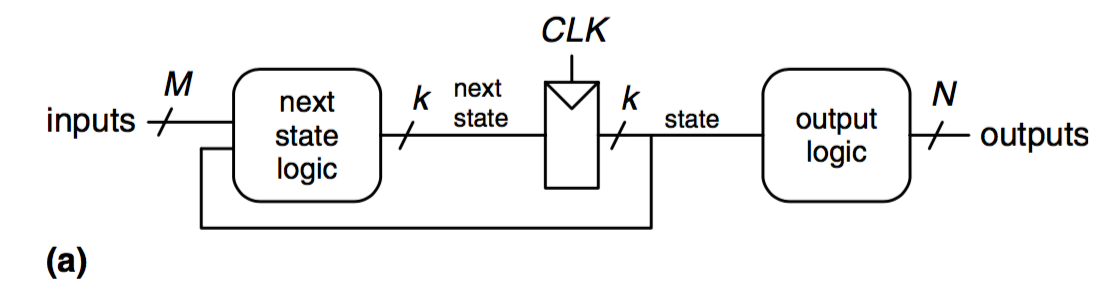
\includegraphics[width = 9cm]{images/seq/moore}
		\end{center}
		\begin{center}
				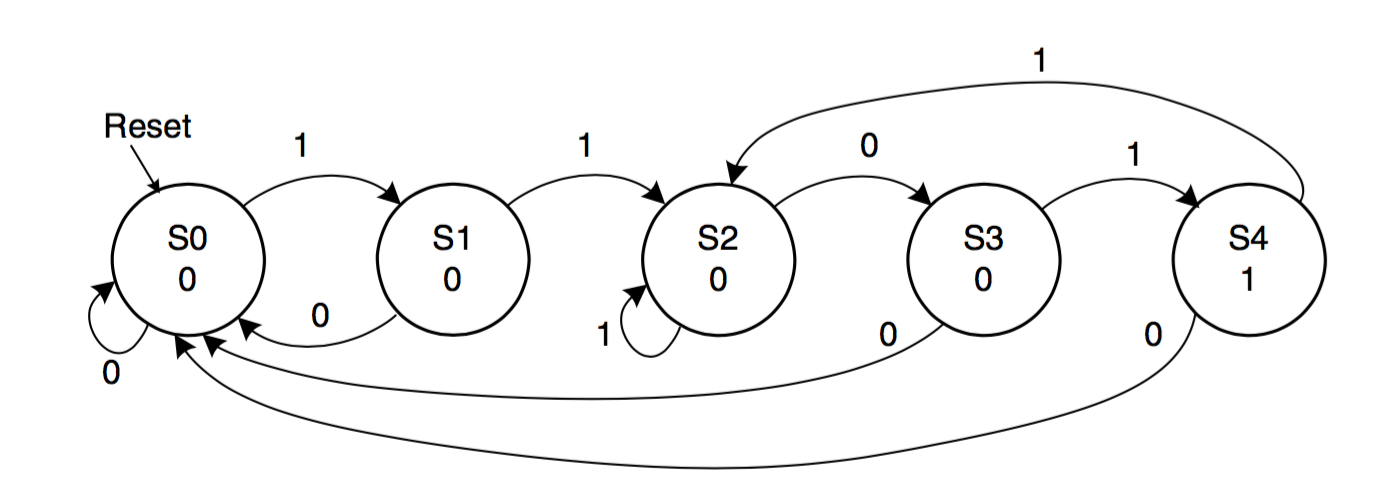
\includegraphics[width = 9cm]{images/seq/moores}
		\end{center}
		And mealy machines, where the ouputs depend on both the current state and the current inputs.
		\begin{center}
				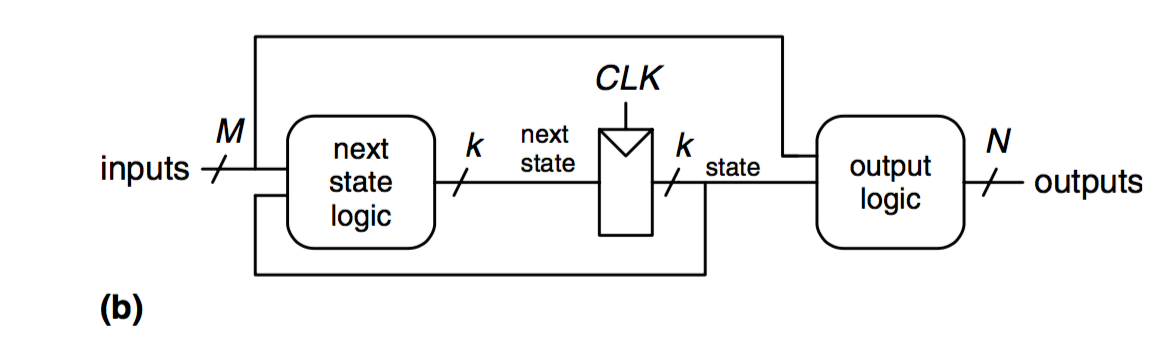
\includegraphics[width = 9cm]{images/seq/mealy}
		\end{center}
		\begin{center}
				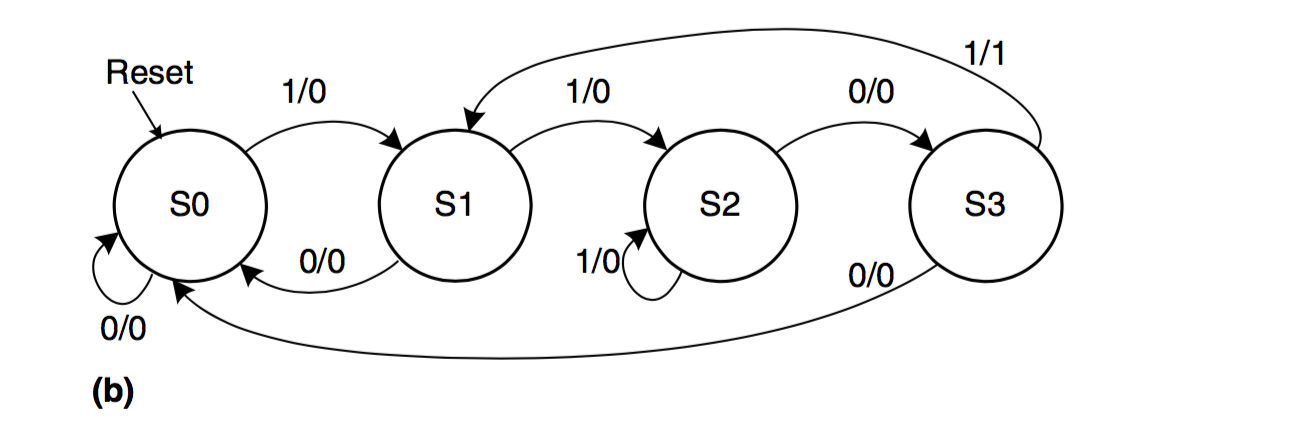
\includegraphics[width = 9cm]{images/seq/mealys}
		\end{center}
		The second picture are the transistion state diagrams, since the mealy machine also depends on the input the arcs also contain the output.\\
	To encode the different states you can use binary encoding, where each state is represented by a binary number. Or one hot encoding where each state is represented by a bit(ex 100, 010 and 001). One hot takes more place but requires fewer gates.\\
	To design a FSM:
	\begin{enumerate}
		\item Identify the inputs and outputs.
		\item Sketch a state transition diagram.
		\item For a Moore machine:
			\begin{enumerate}
				\item Write a state transition table.
				\item Write an output table.
			\end{enumerate}
		\item For a mealy machine:
			\begin{enumerate}
				\item Write a combined state transition and output table.
			\end{enumerate}
		\item Select state encodings—your selection affects the hardware design.
		\item Write Boolean equations for the next state and output logic.
		\item Sketch the circuit schematic.
	\end{enumerate}
	\paragraph{Dynamic discipline}, There is a time during which you cannot write a value to a flip-flop because it is during the clock cycle. For the circuit to sample its input correctly, the input must have stabilized at least some setup time, before the rising edge of the clock and must remain stable for at least some hold time, after the rising edge of the clock. The sum of the setup and hold times is called the aperture time of the circuit, because it is the total time for which the input must remain stable.\\The dynamic discipline states, that the inputs of a synchronous sequential circuit must be stable during the setup and hold aperture time around the clock edge.
	\paragraph{Metastable State}, when the state of the flip-flop is undefined, illegal. The flip-flop will only stay like this for some time and then change to a valid state. Metastable states are due to aschyronous input from users which we can't avoid.
	\paragraph{Synchronizer}
		A sychronizer takes an asychronous input and a clock and with a high probability returns a sychronous output.
	\subsection{Parallelism}
	\paragraph{Latency}, is the time required for a piece of information to pass from start to end of the system
	\paragraph{Throughput}, number of pieces of information the system produces per unit of time.
	\paragraph{Pipelining a circuit}, you can pipeline a circuit by adding registers into the circuit which will let you divide the calculations, like pipelining in PP. Adding a pipeline stage improves throughput at the expense of some latency.
	
	
	
	
	
	
	
	
	
	
	
	
	
	
	
	
	
	
	
	
	
	
	
	\clearpage
	
	
	